\section{Introduction}
\label{sec:introduction}

%\begin{figure}
%  \centering
%  \begin{subfigure}[b]{0.25\textwidth}
%    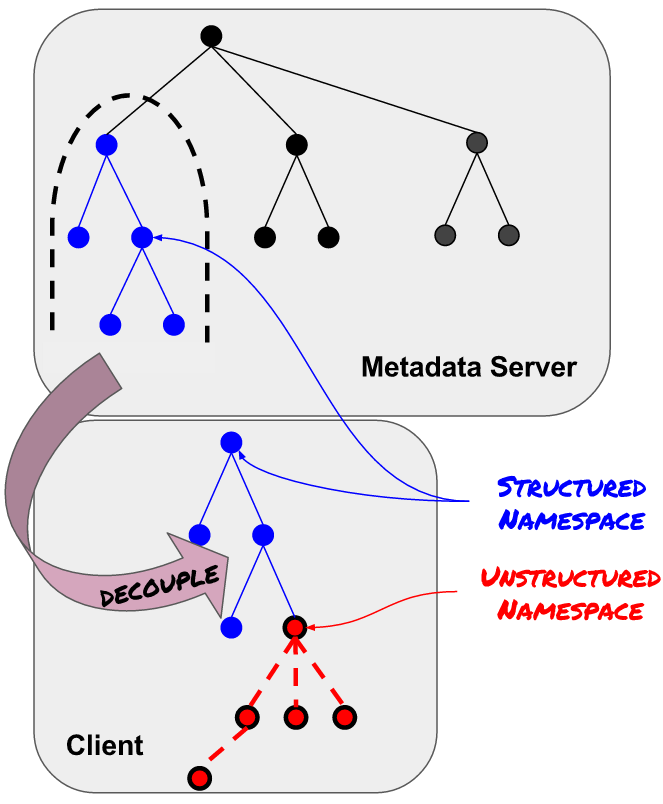
\includegraphics[width=\textwidth]{figures/intro.png}
%   \label{fig:intro}
%  \end{subfigure}
%  ~ 
%  \begin{subfigure}[b]{0.3\textwidth}
%    \begin{tabular}{ r | l }
%      Type         & Overhead       \\\hline\\
%      Structured   & 1 RPC          \\
%      Namespace    & O(1)           \\\\\hdashline\\
%      Unstructured & 1 RPC + Replay \\
%      Namespace    & O(1)           \\\\\hdashline\\
%      Traditional  & \(n\) RPCs     \\
%      Namespace    & O(\(n\))       \\
%    \end{tabular}
%    \\\\\\ % I am a hack
%   \label{table:intro}
%  \end{subfigure}
%  \caption{Clients decouple the file system subtrees and interact with their
%  private copiese locally for high performance. They can specify the structure of
%  the metadata they intend to create (structured namespace) or they can create
%  ad-hoc metadata (unstructured namespace), which is merged later.}
%\end{figure}
%    \caption{Traditional namespaces require at least 1 RPC per metadata
%    operation. Structured namespaces only need the initial RPC so clients/servers
%    understand (and can construct) the namespace.  Unstructured namespaces cannot
%    be parallelized and must replay metadata one by one onto the global namespace}
 
% What is our solution
We propose Tintenfisch, a file system that allows users to succinctly express
the structure and patterns of the metadata they intend to create.  They can
also merge new metadata (that they did not explicitly state up front) into the
global namespace.  Using this semantic knowledge, Tintenfisch can optimize
performance by reducing the number of RPCs needed for:

\begin{itemize}

  \item metadata writes because clients/servers can create metadata
  independently

  \item metadata reads because clients can construct metadata and pull data
  directly from the object store

\end{itemize}

\begin{figure}[t]
  \centering
  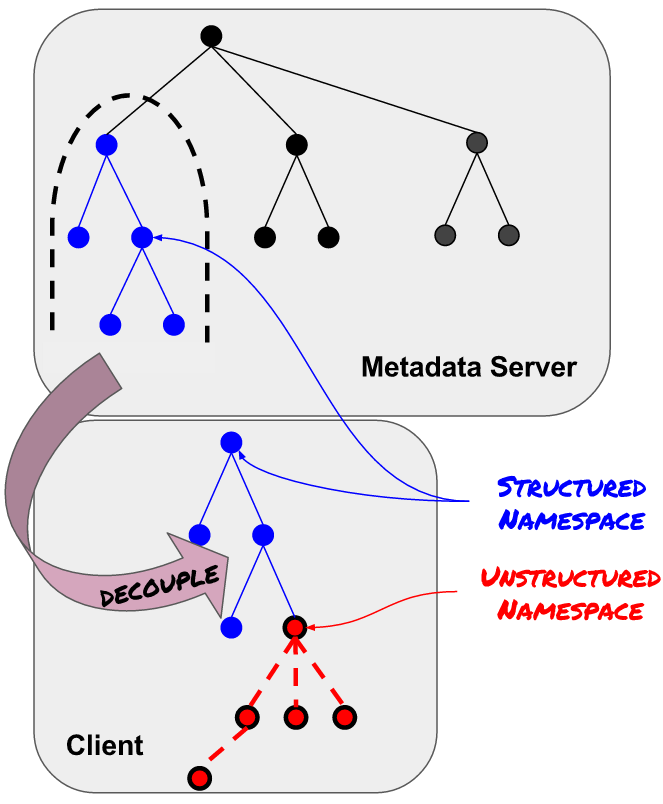
\includegraphics[width=90mm]{figures/intro.png}
  \caption{In (1), clients decouple file system subtrees and interact
with their copies locally for high performance. In (2), clients and
metadata servers generate subtrees using ``namespace schemas", thus reducing
RPC load.  \label{fig:intro}}
\end{figure}

The fundamental insight is that the client and server both understand the final
structure of the file system metadata so there is no need to communicate.  The
idea uses concepts from decoupled namespaces~\cite{zheng:pdsw2014-batchfs,
zheng:pdsw2015-deltafs} and patterned IO~\cite{he:hpdc13-plfs-patterns} to
build a scalable global namespace. Less work is done on the metadata servers
and clients pick up some of the metadata load.  This approach is similar to
predicate push down in databases, where structure is described using XML or
JSON and pushed as predicates to the lower storage
layers~\cite{shel:pc17-pushdown}. It is our hope that Tintenfisch will also be
able to change the representation or structure of the file system metadata
according to the file type or workload.  We have the following contributions:

\begin{itemize}

  \item a prototype implementation that leverages metadata compaction and
  reduces RPC amplification to improve performance

  \item structured and unstructured namespaces, a paradigm that helps
  applications optimize performance by conveying semantic knowledge to the
  storage system.

\end{itemize}
